YouNow gibt in seinen Richtlinien vor, wie man sich verhalten soll. Zusätzlich gibt es die Möglichkeit in seinem Profil Angaben zu verbergen.

\paragraph{Personenbezogene Daten}
YouNow garantiert auf seiner Homepage, keine Daten zu veröffentlichen oder an Dritte weiterzugeben. Jedoch räumt YouNow ein, für Behörden auf Anfrage einer Strafverfolgung nachzukommen. Außerdem schreiben die Richtlinien vor, keine E-Mailadresse, Telefonnummern oder Wohnadressen anderer zu veröffentlichen. Bei Verstoß verspricht YouNow, dies mit einer temporären oder dauerhaften Sperrung zu ahnten.  

\paragraph{Profil}
Für den erstellten Account besteht die Möglichkeit dessen Profil zu bearbeiten (siehe Abbildung~\ref{profil_einstellungen}). Einstellungen in dem Profil sind kein Zwang, denn auch ohne lassen sich alle Funktionen der Plattform nutzen. In den Einstellungen kann man sein Profil- und Hintergrundbild einstellen, einen Nickname und eine Kurzbeschreibung. Außerdem kann hier entschieden werden, ob der richtige Name oder der Nickname in Chats erscheinen soll und ob man seinen Standort preisgeben möchte.

\begin{figure}[h!]
\centering
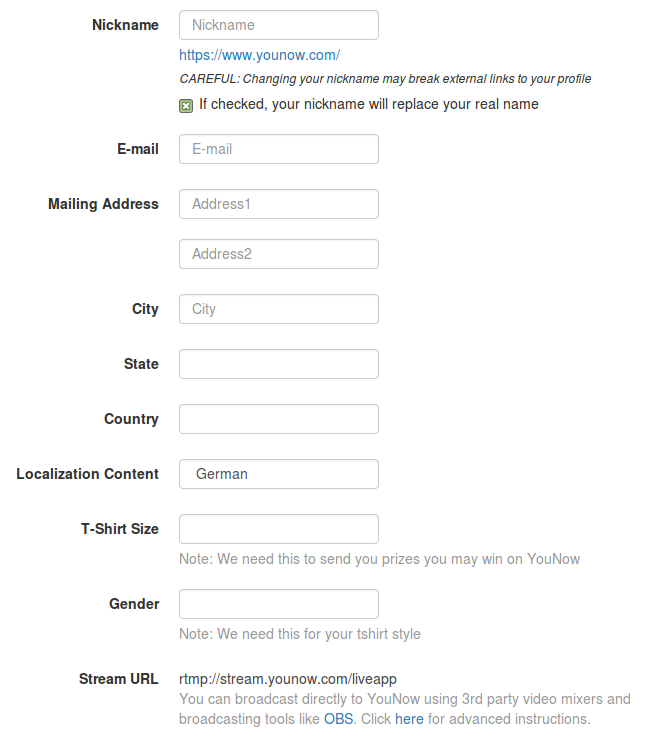
\includegraphics[width=0.5\textwidth]{./resources/younow_profile_settings}
\caption{Einstellungen für das Profil}
\label{profil_einstellungen}
\end{figure} 
